\section{Results}\label{sec:ciResults}

This analysis inspects the high-mass tails of the \ee and \mm invariant mass spectra.
Four signal regions are considered, two each for \ee and \mm selections.
For each signal region, the differential mass distribution in a lower mass control region is fit, in order to produce a background estimate in the signal region.
This section presents the statistical investigation performed on the observation in each signal region, and their physical interpretation.

\subsection{Data}

The data collected and analysed is presented here for each signal region. 
First Table \ref{tab:ciData} presents the data and background expectations, along with the significance of the background-only hypothesis in each SR.

\begin{table}[H]
    \centering
    \begin{tabular}{l   r r@{}l c }
    \toprule
    \multicolumn{1}{c}{SR} & Data & \multicolumn{2}{c}{Background} & Significance \\
    \midrule
    \ee   Constructive & 19 & 12.4 & $\pm1.9$ & ~~~1.28 \\
    \ee   Destructive  & 2  & 3.1  & $\pm1.1$  & --~0.72 \\
    \midrule
    \mm Constructive & 6  & 9.6  & $\pm2.1$  & --~0.99 \\
    \mm Destructive  & 1  & 1.4  & $\pm0.9$  & --~0.58 \\
    \bottomrule
    \end{tabular}
    \caption{The dielectron and dimuon event yields for the data, the expected background and the respective significance in the different SRs used in the analysis.  The p-value of each observation is defined as the probability, given the background-only hypothesis, of an observation at least as large as that seen in the data.  The significance is the Gaussian cumulative density function of the p-value, and negative significances correspond to deficits. }
    \label{tab:ciData}
\end{table}

Small deficits compared to the expected background are seen in the \mm SRs, along with the \ee destructive SR.
A moderate excess is observed in the \ee constructive SR.
None of the these significances are judged to be significant enough to reject the background-only hypothesis.

\afterpage{
\begin{figure}[h!]
\centering
\subfloat[][]{{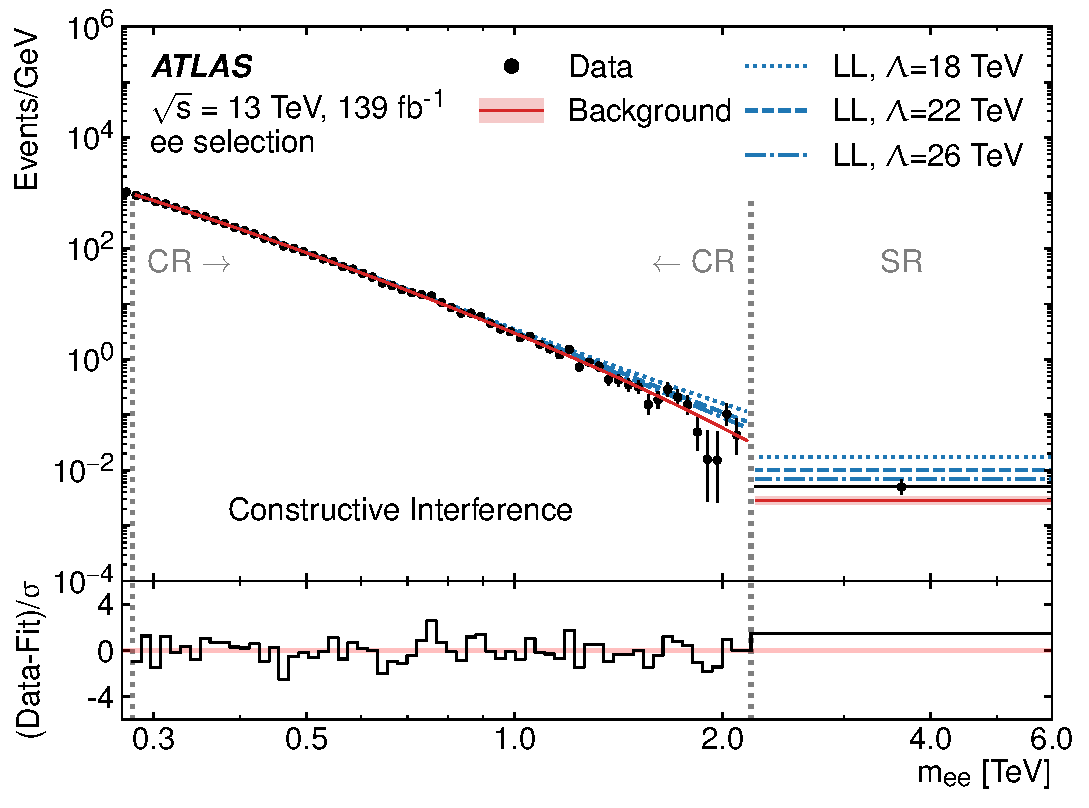
\includegraphics[width=0.5\textwidth]{figures/ci/results/fig_02a.pdf}}} % will be fig_02a.pdf
\subfloat[][]{{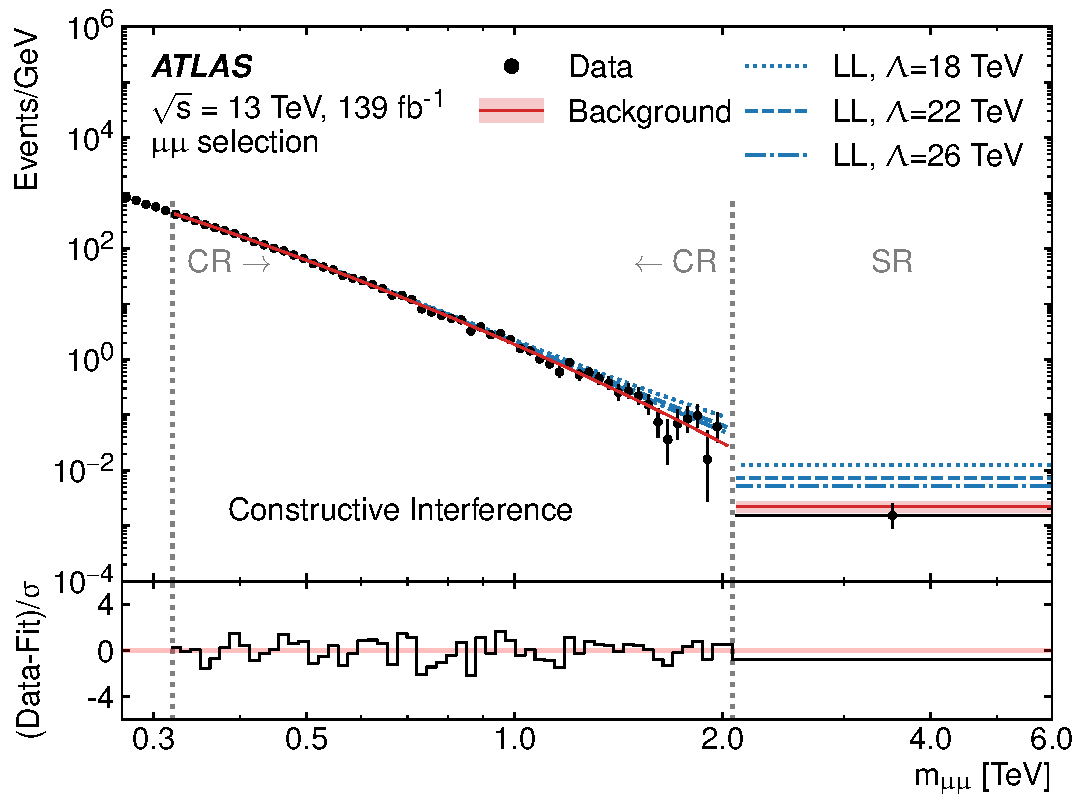
\includegraphics[width=0.5\textwidth]{figures/ci/results/fig_02b.pdf}}}\\ % will be fig_02b.pdf
\subfloat[][]{{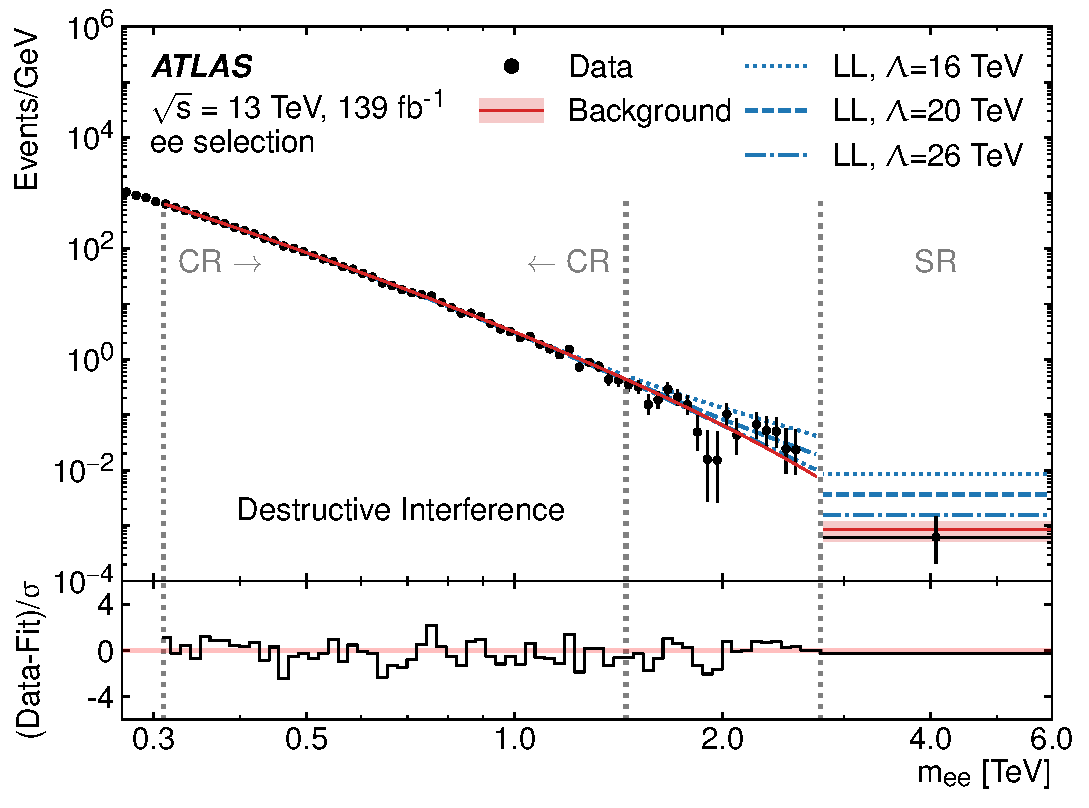
\includegraphics[width=0.5\textwidth]{figures/ci/results/fig_02c.pdf}}} % will be fig_02c.pdf
\subfloat[][]{{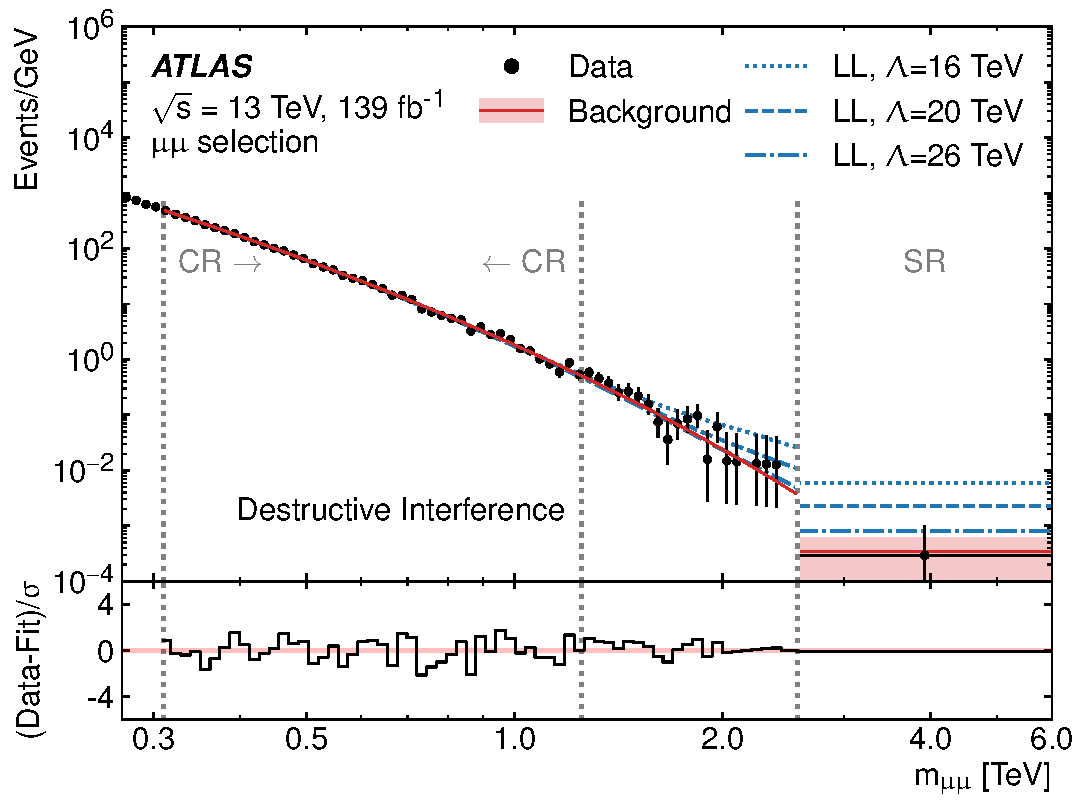
\includegraphics[width=0.5\textwidth]{figures/ci/results/fig_02d.pdf}}} % will be fig_02d.pdf
\caption{
Distributions of the invariant mass of dilepton pairs passing the full selection for dielectrons (left) and dimuons (right), and showing CR and SR for constructive interference (top) and destructive interference (bottom).
Figures (c) and (d) show the region between the SR and CR, but this is not used by the fit.
The data points are plotted at the centre of each bin as the number of events divided by the bin width, which is constant in $\log{(m_{\ell\ell})}$.
The error bars indicate statistical uncertainties only.
A few CI benchmark signal shapes are shown, scaled to the data luminosity and superimposed by subtracting the LO DY component and adding the resulting shape to the background shape obtained from the fit.
These signals have LL chirality with $\Lambda=$ 18, 22, and 26~TeV for the constructive case and $\Lambda=$16, 20, and $26$~TeV for the destructive case.
The background-only fit is shown in solid red, with the light red area being its uncertainty.
The boundaries of the CR and SR corresponding to the signals used are shown in dotted vertical lines for reference and marked by arrows.
%In the destructive interference case, the signal shapes do not differ much on the scale used for these plots.
The differences between the data and the fit results in units of standard deviations of the statistical uncertainty are shown in the bottom panels.
}
\label{fig:ciDist}
\end{figure}
\clearpage
}

The signal regions and control regions are illustrated in the plots of Figure \ref{fig:ciDist}.
There are a couple of points to remark on.
First, the agreement between the fitted background function and the data is consistent and good in each CR.
The agreement is also quite good in the gap between the CR and destructive SRs.
Next the excesses and deficits listed in Table \ref{tab:ciData} appear in the signal regions of the plots.
For comparison, the predictions of several CI signal models are imposed on top of the background estimate.

The parameters of the fitted background shape are given in table \ref{tab:fitpars}.
\begin{table}[htp]
\centering
\caption{Parameters for the functional form given in Equations \ref{eqn:ciBkgEe} and \ref{eq:ciBkgMm}. The uncertainties are statistical only.}
{\footnotesize
 \begin{tabular}{l  r@{}c@{}l r@{}c@{}l  r@{}c@{}l r@{}c@{}l }
\toprule
Parameter  &  \multicolumn{3}{c}{\ee Constructive} &  \multicolumn{3}{c}{\ee Destructive} &  \multicolumn{3}{c}{\mm Constructive} &  \multicolumn{3}{c}{\mm Destructive} \\
\midrule
 Normalization & \multicolumn{3}{c}{$(6.17 \pm 0.02)\times 10^\text{-3}$} & \multicolumn{3}{c}{$(7.87\pm 0.03)\times 10^\text{-3}$} & \multicolumn{3}{c}{$(6.90\pm 0.03)\times 10^\text{-6}$} & \multicolumn{3}{c}{$(4.39\pm 0.02)\times 10^\text{-7}$} \\
 b (fixed) & \multicolumn{3}{c}{6.1} & \multicolumn{3}{c}{6.1} & \multicolumn{3}{c}{1.3} & \multicolumn{3}{c}{1.3} \\
 % c (fixed) & \multicolumn{3}{c}{1/2} & \multicolumn{3}{c}{1/2} & \multicolumn{3}{c}{1/3} & \multicolumn{3}{c}{1/3} \\
 $p_0$ &  ~~~~-12.2   & $\pm$ & 0.1       & ~~~~~-12.1  &$\pm$& 0.1   & ~~~~~-14.9  &$\pm$& 0.2   & ~~~~~-17.0 &$\pm$& 0.2 \\
 $p_1$ &  ~~~~-4.14   & $\pm$ & 0.02      & ~~~~~-4.16  &$\pm$& 0.03  & ~~~~~-4.42 &$\pm$& 0.04  &  ~~~~~-4.70 &$\pm$& 0.04 \\
 $p_2$ &  ~~~~-0.948  & $\pm$ & 0.005     & ~~~~~-0.945 &$\pm$& 0.006 & ~~~~~-0.927 &$\pm$& 0.008 & ~~~~~-0.846 &$\pm$& 0.008 \\
 $p_3$ &  ~~~~-0.0840 & $\pm$ & 0.0008    & ~~~~~-0.082 &$\pm$& 0.001 & ~~~~~-0.081 &$\pm$& 0.001 & ~~~~~-0.064 &$\pm$& 0.001 \\
\bottomrule\end{tabular}}
\label{tab:fitpars}
\end{table}

Although the background expectations from simulation are not used explicitly for hypothesis tests, they are provided in Table \ref{tab:ciMcVsFit} along with the nominal background expectations.
The systematic uncertainty on the simulated \nbkg takes into account experimental and theoretical uncertainties, however these are not well known in the SR.
No significant difference between the nominal background estimate and the simulated background estimate.

\begin{table}[h!]
\centering
\caption{Comparison between the background estimate in the SR, as derived from fitting the data ($N_\text{fit}$), and the estimation from simulated background ($N_\text{sim}$). The yields observed in data ($N_\text{obs}$) are also given. All systematic uncertainties are included.}
\begin{tabular}{l | r r r }\toprule
SR & $N_\text{sim}\pm\sigma_\text{sim}$ & $N_\text{fit}\pm\sigma_\text{fit}$ & $N_\text{obs}$ \\
\hline
\ee Constructive   & $13.3  \pm 1.9$  & $12.4 \pm 1.9$ & 19 \\
\ee Destructive    & $2.9   \pm 0.6$  & $3.1  \pm 1.1$ & 2  \\ % fixed ee
\mm Constructive & $11.9  \pm 2.8$  & $9.6  \pm 2.1$ & 6  \\
\mm Destructive  & $3.3   \pm 1.0$  & $1.4  \pm 0.9$ & 1  \\
\bottomrule\end{tabular}\\ %remember cline{1-2}
\label{tab:ciMcVsFit}
\end{table}

A further comparison of the background differential shapes made in Figure \ref{fig:ciCiFitVsMc}.
These plots shows a comparison between the fitted background function, and the simulated background distribution in both the CR and SR.
The fitted background function is produced using the fit to data, not the simulation.

\begin{figure}[!htpb]
\centering
\subfloat[][]{{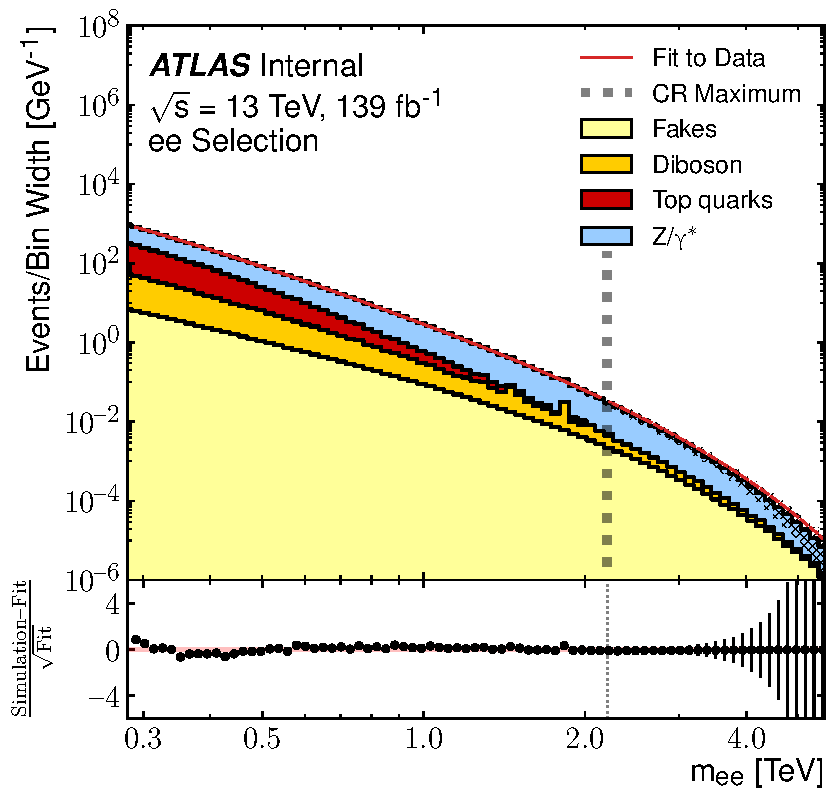
\includegraphics[width=0.45\textwidth]{figures/ci/results/figaux_08a.pdf}}}
\subfloat[][]{{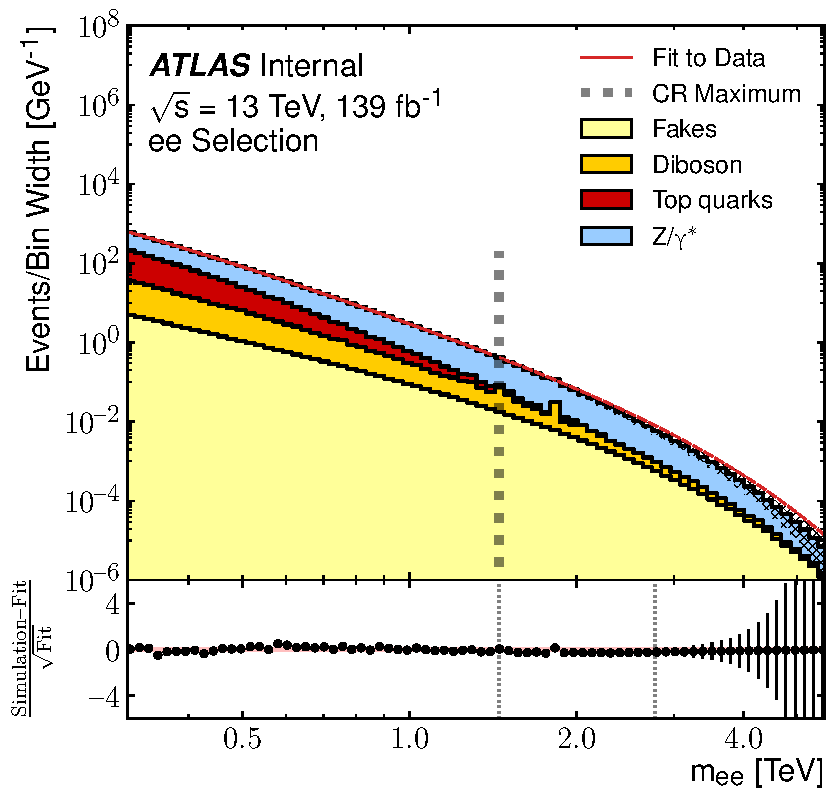
\includegraphics[width=0.45\textwidth]{figures/ci/results/figaux_08b.pdf}}} \\
\subfloat[][]{{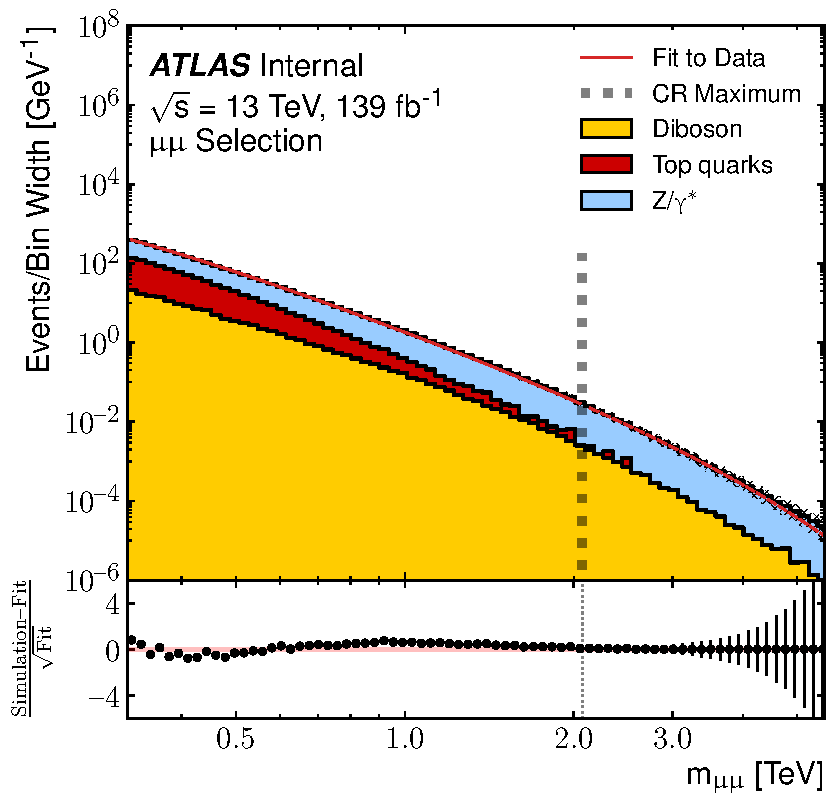
\includegraphics[width=0.45\textwidth]{figures/ci/results/figaux_08c.pdf}}}
\subfloat[][]{{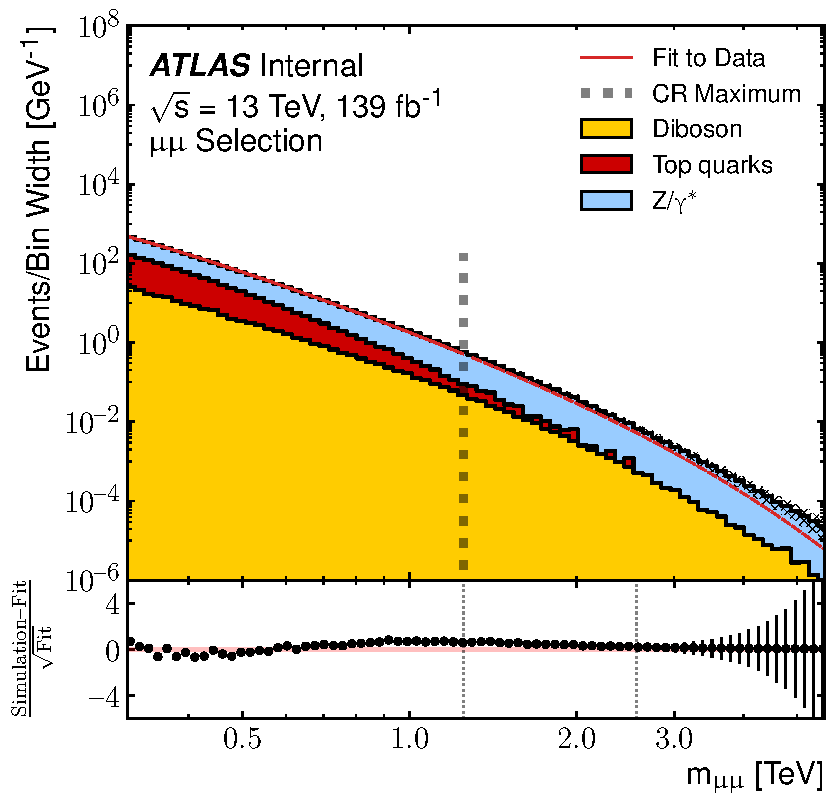
\includegraphics[width=0.45\textwidth]{figures/ci/results/figaux_08d.pdf}}}
\caption{Fits performed on data (red) are compared to the background simulation. The background simulation is used only to study performance and systematics. The uncertainties on the background simulation are theory only, and are provided as a rough estimate.
Shown for \ee constructive (a), \ee destructive (b), \mm constructive (c), and \mm destructive (d).}
\label{fig:ciCiFitVsMc}
\end{figure}




\subsection{Limits on signal events}\label{sec:limNSig}

\begin{figure}[h!]
\begin{center}
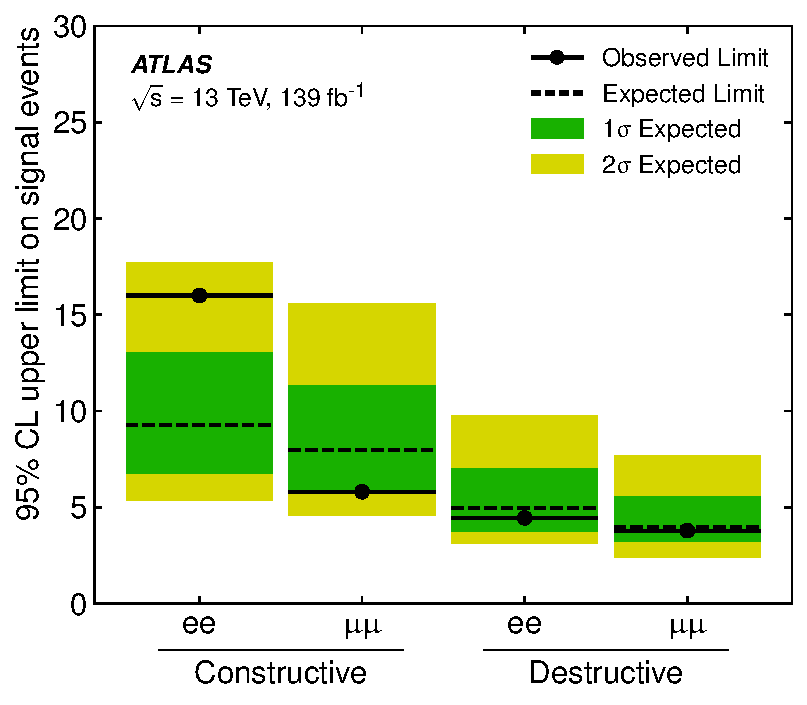
\includegraphics[width=0.5\linewidth]{figures/ci/results/fig_03a.pdf}
\end{center}
\vspace{-.4cm}
\caption{Limits on the number of signal events in the respective signal region for each model. }
\label{fig:ciCiLimNSig}
\end{figure}

In the absence of significant deviations of the data from the background expectation, the observations are used to set limits on signal production in each SR.
The limits in this section use the hypotheses defined in Equations \ref{eqn:ciNullLikelihoodNSig} and \ref{eqn:ciAltLikelihoodNSig}.
The parameter of interest is the number of signal events to pass the event selection, \nsig.
This is trivially converted to limits on the visible component of a signal production mechanism, \xsbr, with the division by the integrated luminosity.
The expected and observed upper limits on both \nsig and \xsbr at 95\% confidence level are given in Table \ref{tab:ciNsigLimits}.
Because these limits do not make strict assumptions about the signal production mechanism, they can be directly reinterpreted for different new physics models that predict dilepton production in the SRs.

\begin{table}[h!]
\begin{center}
\caption{The observed model-independent upper limit at 95\% CL on the visible cross-section times branching fraction \xsbr and the number of signal events $(N_\textrm{sig})$ in the dielectron and dimuon SRs used in the analysis.}
{
\begin{tabular}{l  c c  c d{1}  d{1} c d{1} c d{1} c}
% \Xhline{2\arrayrulewidth}
\toprule
\multicolumn{1}{c}{\multirow{2}{*}{SR}}           & \multicolumn{2}{c}{Limit on \xsbr [fb]} & \multicolumn{2}{c}{Limit on \nsig} \\
             &  {Exp.} & {Obs.}  & {Exp.} & \multicolumn{1}{r}{{Obs.}} \\
\midrule
\ee   Constructive & 0.067   & 0.115 & 9.3  & 16.0 \\
\ee   Destructive  & 0.036   & 0.032 & 5.0  & 4.4  \\
\midrule
\mm Constructive & 0.057   & 0.042 & 8.0 & 5.8   \\
\mm Destructive  & 0.029   & 0.027 & 4.0 & 3.8   \\
\bottomrule
\end{tabular}
}
\label{tab:ciNsigLimits}
\end{center}
\end{table}

The results in Table \ref{tab:ciNsigLimits} are illustrated and complemented by Figure \ref{fig:ciCiLimNSig}.
This plot shows the observed limits on \nsig in each SR.
The expected limits, which are the limits expected when the observed yield equals the background expectation, are shown as well.
Bands of $\pm1\sigma$ and $\pm2\sigma$ intervals are drawn around each expected limit, which contain 68\% and 95\% of the expected limits generated by pseudo-observations.

The excesses and deficits from Table \ref{tab:ciData} are seen to manifest themselves in this plot.
The excess of \ee events in the constructive SR have weakened the corresponding observed limit.
In the other limits, the deficits of events are seen to have allowed slightly stronger limits than expected.
None of the observed limits differ significantly from the expected limits. 
\footnote{This statement is in fact distinct from the statement given earlier that none of the observations are significantly different from the expected background. The limits are computed using \cls, while the earlier statement considers only the p-value of the background-only hypothesis. In any case, both statements share a compatible message.}

\begin{table}[h!]
\begin{center}
\caption{The expected yields for a few CI signal points (LL chirality only) are listed along with the signal acceptance times efficiency \acceff values for reference.}
{
\begin{tabular}{l  c c  c d{1}  d{1} c d{1} c d{1} c}
% \Xhline{2\arrayrulewidth}
\toprule
\multicolumn{1}{c}{\multirow{3}{*}{SR}} &  \multicolumn{2}{c}{$\Lambda=20~$TeV} & \multicolumn{2}{c}{$\Lambda=30~$TeV}  & \multicolumn{2}{c}{$\Lambda=40~$TeV} \\
             &  \nsig & \acceff & \nsig & \acceff & \nsig & \acceff \\
\midrule
\ee   Constructive & 39.1 & 0.69  & 10.3 & 0.69  &  4.4  & 0.69 \\
\ee   Destructive  & 9.6  & 0.70  & 1.0  & 0.70  & -0.1 & 0.69 \\
\midrule
\mm Constructive & 28.5 & 0.43  & 7.7  & 0.43  &  3.4  & 0.43 \\
\mm Destructive  & 7.1  & 0.43  & 0.6 & 0.42  & -0.2 & 0.44 \\
\bottomrule
\end{tabular}
}
\label{tab:ciYields_sig}
\end{center}
\end{table}

The limits in Table \ref{tab:ciNsigLimits} are placed in context with the signal yields for CI models in Table \ref{tab:ciYields_sig}.
The signal models that predict signal event yields above above the corresponding limits on \nsig in Table \ref{tab:ciNsigLimits} are excluded.
Next to each \nsig yield is the product of the detector acceptance and efficiency: the fraction of produced signal events expected to be reconstructed in the SR.
% reinterpretation
Although these values are provided for CI signal shapes, an inspection of their variance shows that these are relatively shape independent.
The number of \nsig events to appear in a SR for a new physics model may be approximated by multiplying the number of events produced according to the model by the corresponding \xsbr fraction given.
Then, this \nsig can be compared to the limits on \nsig to determine whether the observed data is incompatible with the model under consideration.

\subsection{Limits on $\Lambda$}
\label{sec:limLambda}

The observations in the signal regions are incompatible with many contact interaction models.
The following tables assess which signal models may be counted as excluded.
To this end, the hypotheses defined in \ref{eqn:ciNullLikelihood} and \ref{eqn:ciAltLikelihood} are compared to the observed data.
Both the single lepton channel hypotheses (\ee and \mm), as well as the dilepton combination (\ll), are considered.
The observed and expected limits set at 95\% confidence level on the contact interaction scale \lam are shown in Table \ref{tab:lambdaLimits1}.
The highest limit is the exclusion of \lam below 35.8~TeV for \ll constructive CI with left-left chirality.
Also notable is the exclusion of \lam below 28.8~TeV for \ll destructive CI with left-right and right-left chiralities.

\begin{table}[h!]
\begin{center}
\caption{Expected and observed lower limits at 95$\%$ CL on $\Lambda$ in TeV for the dielectron and dimuon channels separately and the combined dilepton channel and for CI signal hypotheses with constructive and destructive interference and different chiralities.}
{\begin{tabular}{c c c c c c c c c c c c}\toprule
Int. & Channel & Exp./Obs. & LL & LR & RL & RR \\
\midrule
\multirow{3}{*}[-1.5em]{\begin{sideways}Constructive\end{sideways}} & \multirow{2}{*}{$ee$} & Expected & 31.1 & 28.9 & 28.7 & 30.9 \\
& & Observed & 26.1 & 24.7 & 24.6 & 26.0 \\
\cmidrule{2-7}
 & \multirow{2}{*}{$\mu\mu$} & Expected & 29.2 & 27.1 & 27.0 & 29.0 \\
& & Observed & 32.7 & 30.0 & 29.8 & 32.6 \\
\cmidrule{2-7}
 & \multirow{2}{*}{$\ell\ell$} & Expected & 37.6 & 34.0 & 33.7 & 37.3 \\
& & Observed & 35.8 & 32.5 & 32.3 & 35.5 \\
\midrule
\multirow{3}{*}[-1.5em]{\begin{sideways}Destructive\end{sideways}} & \multirow{2}{*}{$ee$} & Expected & 23.0 & 24.4 & 24.4 & 23.2 \\
& & Observed & 23.5 & 25.1 & 25.1 & 23.7 \\
\cmidrule{2-7}
 & \multirow{2}{*}{$\mu\mu$} & Expected & 22.0 & 23.6 & 23.6 & 22.2 \\
& & Observed & 22.3 & 23.9 & 23.9 & 22.5 \\
\cmidrule{2-7}
 & \multirow{2}{*}{$\ell\ell$} & Expected & 25.6 & 28.0 & 28.0 & 25.9 \\
& & Observed & 26.0 & 28.8 & 28.8 & 26.5 \\
\bottomrule\end{tabular}}
\label{tab:lambdaLimits1}
\end{center}
\end{table}

The limits shown in table \ref{tab:lambdaLimits1} are set without theoretical uncertainty on the signal model.
The choice of the signal model corresponds to the choice of the signal+background hypothesis, and consequently there is no uncertainty related to that definition.
Alternative signal models, corresponding to possible theoretical variations, may also be used to set limits on \lam.
These alternative models predict either enhanced or diminished signal event event yields to the SR.
Two models are considered: one with $+1\sigma$ theoretical increase to the event yield, and one with $-1\sigma$ theoretical reduction to the event yield.
The limits set on these alternative models are given in Table \ref{tab:limits_on_lambda_theoryUp} for $+1\sigma$ Table \ref{tab:limits_on_lambda_theoryDn} for $-1\sigma$.

\begin{table}[htp]
\begin{center}
\caption{Expected and observed lower limits at 95$\%$ CL on $\Lambda$ in TeV for the dielectron and dimuon channels separately
and for the combined electron-muon channel, for a theoretical variation on the CI signal hypotheses with constructive
and destructive interference and different chiralities.
The CI signal hypothesis has been increased by $+1\sigma_\text{s}^\text{Theory}$.}
{\begin{tabular}{r c c c c c c c c c c c}\toprule
Int. & Channel & Exp./Obs. & LL & LR & RL & RR \\
\midrule
\multirow{3}{*}[-1.5em]{\begin{sideways}Constructive\end{sideways}} & \multirow{2}{*}{$ee$} & Expected & 31.9 & 29.4 & 29.4 & 31.7 \\
& & Observed & 26.8 & 25.2 & 25.2 & 26.6 \\
\cmidrule{2-7}
 & \multirow{2}{*}{$\mu\mu$} & Expected & 31.1 & 28.8 & 28.6 & 30.9 \\
& & Observed & 35.1 & 31.8 & 31.6 & 34.7 \\
\cmidrule{2-7}
 & \multirow{2}{*}{$\ell\ell$} & Expected & 39.6 & 35.6 & 35.4 & 39.3 \\
& & Observed & 38.6 & 34.7 & 34.4 & 38.2 \\
\midrule
\multirow{3}{*}[-1.5em]{\begin{sideways}Destructive\end{sideways}} & \multirow{2}{*}{$ee$} & Expected & 23.3 & 24.9 & 24.9 & 23.5 \\
& & Observed & 23.8 & 25.5 & 25.5 & 24.0 \\
\cmidrule{2-7}
 & \multirow{2}{*}{$\mu\mu$} & Expected & 23.2 & 25.2 & 25.1 & 23.5 \\
& & Observed & 23.5 & 25.4 & 25.4 & 23.7 \\
\cmidrule{2-7}
 & \multirow{2}{*}{$\ell\ell$} & Expected & 26.5 & 29.2 & 29.2 & 26.9 \\
& & Observed & 26.9 & 29.9 & 29.9 & 27.3 \\
\bottomrule\end{tabular}}\\
\label{tab:limits_on_lambda_theoryUp}
\end{center}
\end{table}

\begin{table}[htp]
\begin{center}
\caption{Expected and observed lower limits at 95$\%$ CL on $\Lambda$ in TeV for the dielectron and dimuon channels separately
and for the combined electron-muon channel, for a theoretical variation on the CI signal hypotheses with
constructive and destructive interference and different chiralities.
The CI signal hypothesis has been reduced by $-1\sigma_\text{s}^\text{Theory}$.}
{\begin{tabular}{r c c c c c c c c c c c}\toprule
Int. & Channel & Exp./Obs. & LL & LR & RL & RR \\
\midrule
\multirow{3}{*}[-1.5em]{\begin{sideways}Constructive\end{sideways}} & \multirow{2}{*}{$ee$} & Expected & 30.3 & 28.1 & 28.0 & 30.0 \\
& & Observed & 25.5 & 24.0 & 24.0 & 25.3 \\
\cmidrule{2-7}
 & \multirow{2}{*}{$\mu\mu$} & Expected & 26.7 & 25.1 & 25.0 & 26.6 \\
& & Observed & 30.3 & 27.9 & 27.7 & 30.0 \\
\cmidrule{2-7}
 & \multirow{2}{*}{$\ell\ell$} & Expected & 35.4 & 32.1 & 31.9 & 35.0 \\
& & Observed & 32.7 & 30.1 & 30.0 & 32.5 \\
\midrule
\multirow{3}{*}[-1.5em]{\begin{sideways}Destructive\end{sideways}} & \multirow{2}{*}{$ee$} & Expected & 22.5 & 23.9 & 23.9 & 22.7 \\
& & Observed & 23.0 & 24.5 & 24.5 & 23.3 \\
\cmidrule{2-7}
 & \multirow{2}{*}{$\mu\mu$} & Expected & 18.7 & 18.3 & 18.3 & 18.7 \\
& & Observed & 20.7 & 21.8 & 21.7 & 20.8 \\
\cmidrule{2-7}
 & \multirow{2}{*}{$\ell\ell$} & Expected & 24.5 & 26.5 & 26.5 & 24.8 \\
& & Observed & 25.1 & 27.4 & 27.4 & 25.4 \\
\bottomrule\end{tabular}} \\
\label{tab:limits_on_lambda_theoryDn}
\end{center}
\end{table}

The limits on \lam shown in Table \ref{tab:lambdaLimits1} are shown in the plots of Figure \ref{fig:limLamb}.
The plots (a) and (b) show the limits set in the \ee and \mm channels.
Four limits, corresponding to the four chirality combinations, are set in each SR.
Since each of these limits relies on the same observation, the pattern of the observed limits with respect to the expectation are the same in each SR.
For example, the excess of dielectron events in the \ee constructive SR leads to lower limits in the left side of Figure \ref{fig:limLamb} (a).
The deficits in the other SRs lead to slightly stronger limits on destructive \lam in plot (a), and also stronger \mm limits in plot (b).

Next, Figure \ref{fig:limLamb} (c) shows the limits on dilepton models using the statistical combination of both \ee and \mm channels.
The combination leads to higher expected limits for all chiralities and interferences.
Since both \ee and \mm destructive limits are stronger than expected, the dilepton combination for destructive limits are stronger as well.
This is not the case for the combined constructive limits, where the excess in the \ee SR works against the deficit in the \mm SR.
Here, the combined limit is weaker than the expectation.
This is a result of the relatively small systematic uncertainties for the \ee channel, which cause the dielectron observation to dominate the combination.

\afterpage{
\begin{figure}[h!]
\captionsetup[subfigure]{position=b}
\centering
\subfloat[][]{{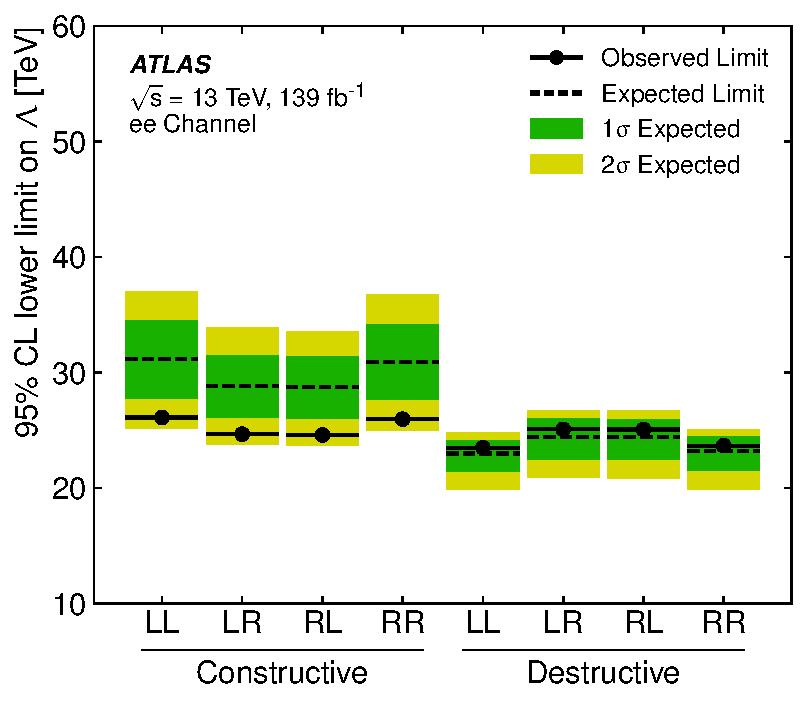
\includegraphics[width=0.5\textwidth]{figures/ci/results/fig_04b.pdf}}}
\subfloat[][]{{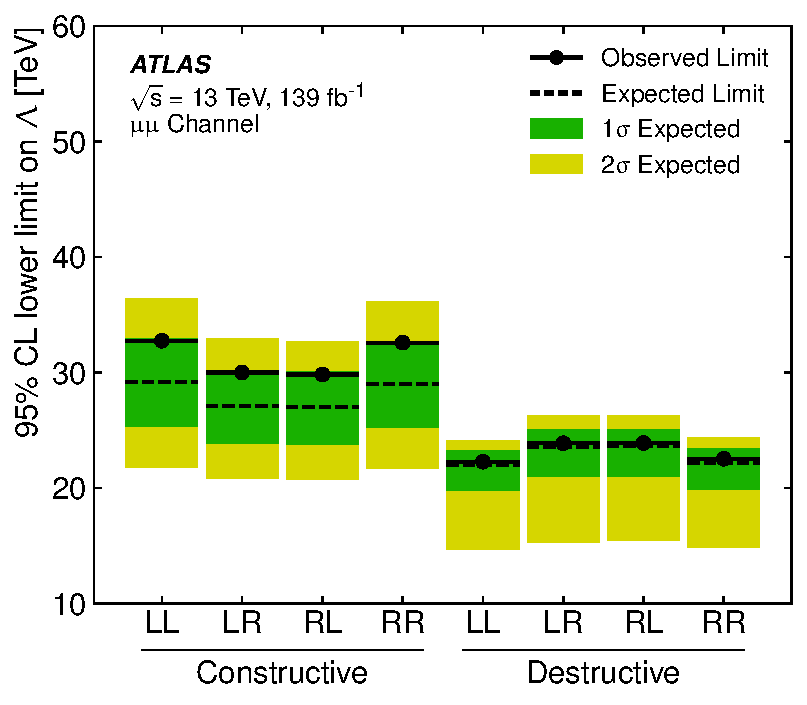
\includegraphics[width=0.5\textwidth]{figures/ci/results/fig_04a.pdf}}} \\
\vspace{2em}
\subfloat[][]{{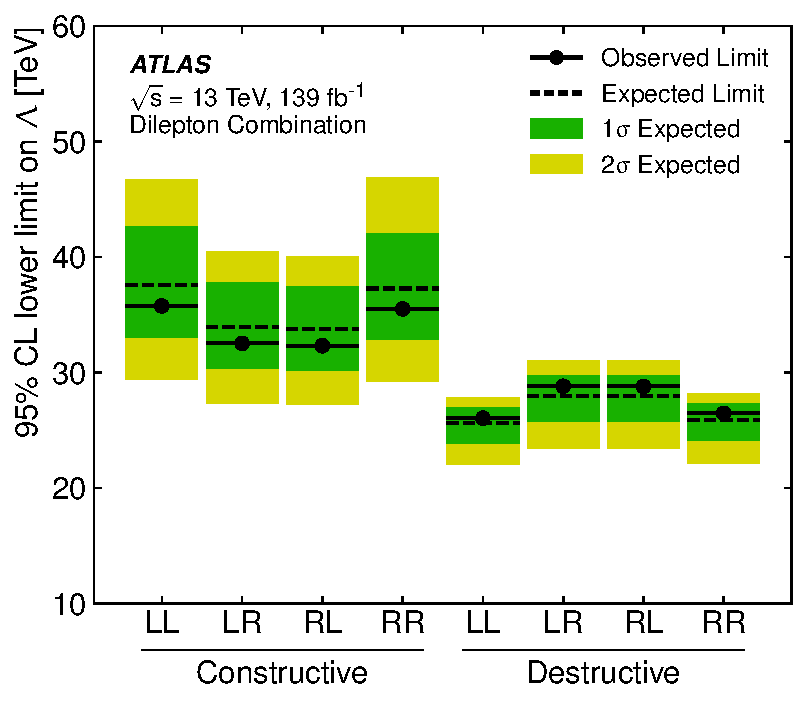
\includegraphics[width=0.5\textwidth]{figures/ci/results/fig_04c.pdf}}}
\vspace{1em}
\caption{Limits on the contact interaction scale \lam for the (a) the \ee channel, (b) the \mm channel, and (c) the statistical combination of both channels..
For each interference and chiral model shown in the bottom axis, the expected and observed limits are shown. The dotted line shows the expected limits and the green and yellow error bars show the 1 and $2\sigma$ uncertainty bands on the expectation. The black points show the observed limits.}
\label{fig:limLamb}
\end{figure}
\clearpage
}

